\documentclass[a4paper, 12pt]{article}

\usepackage{cmap}
\usepackage{mathtext} 
\usepackage[T2A]{fontenc}
\usepackage[utf8]{inputenc}
\usepackage[english,russian]{babel}	

\usepackage{amsfonts,amssymb,amsthm,mathtools}
\usepackage{amsmath}
\usepackage{icomma} 

\usepackage{graphicx} 
\graphicspath{{Picturies/}}
\usepackage{wrapfig}

\usepackage{array,tabularx,tabulary,booktabs}
\usepackage{longtable}
\usepackage{multirow}

\usepackage{caption}
\captionsetup{labelsep=period}

\renewcommand{\phi}{\varphi}
\newcommand{\eps}{\varepsilon}
\newcommand{\parag}[1]{\paragraph*{#1:}}

\newcounter{Points}
\setcounter{Points}{1}
\newcommand{\point}{\arabic{Points}. \addtocounter{Points}{1}}

\author{Вязовцев Андрей, Б01-005}
\date{9.03.21}
\title{Лабораторная работа 2.4.1. Определение теплоты испарения жидкости}

\begin{document}

\maketitle

\parag {Цель работы}
1) измерение давления насыщенного пара жидкости при разной температуре; 2) вычисление по полученным данным теплоты испарения с помощью уравнения Клапейрона-Клаузиуса

\parag {В работе используются}
термостат; герметический сосуд, заполненный исследуемой жидкостью; отсчётный микроскоп.

\parag {Теоритическая справка} ~\\

Фаза вещества --- макроскопическая физическая однородная часть вещества, отделённая от остальных частей системы границами раздела, так что она может быть извлечена из системы механическим путём.

Для рассмотрения состояния равновесия различных фаз удобно ввести термодинамический потенциал $\Phi$. Он является функцией состояния и равен:

\[
    \Phi = U + PV - TS
\]

Пусть система состоит из двух фаз. Из соображений равновесия удельные термодинамические потенциалы $\phi$ должны быть равны для них:

\[
    \phi_1 (P, T) = \phi_2 (P, T)
\]

Из этого следует уравнение Клапейрона-Клаузиуса:

\[
    \frac{dP}{dT} =   \frac{q}{T(v_2 - v_1)}
\]

Где $v_1$ и $v_2$ --- удельные объёмы фаз вещества, а $q$ --- удельная теплота фазового перехода из состояния 1 в состояние 2.

Для испарения это уравнение можно переписать в виде:

\[
    \frac{dP}{dT} = \frac{L}{T (V_2 - V_1)}
\]

Где $P$ --- давление насыщенного пара при $T$, $T$ --- абсолютная температура жидкости и права, $L$ --- теплота испарения жидкости, $V_2$, $V_1$ --- объёмы пара и жидкости соответственно.

Так же для пара можно записать уравнение Ван-дер-Ваальса для $1$ моля газа:

\[
    \left(P + \frac{a}{V_2^2}\right) (V_2 - b) = RT
\]

Значения $V_1$, $V_2$, $a$ и $b$ можно узнать из данной таблицы:

\begin{figure}[!h]
    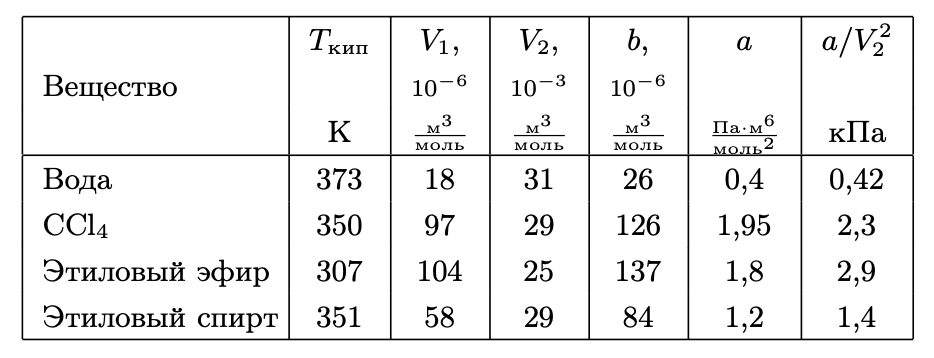
\includegraphics[scale = 0.7]{Constants}
\end{figure}

Как видно отсюда, $V_1$, $b$, и $\dfrac{a}{V_2^2}$ --- малые величины, ими в уравнениях можно пренебречь. Таким образом, уравнение Ван-дер-Ваальса станет уравнением Менделеева-Клапейрона. А конечное выражение для $L$ запишется так:

\begin{equation} \label{eq:L}
    L = -R \cdot \frac{d(\ln P)}{d(1/T)}
\end{equation}

\parag {Экспериментальная установка} ~

\begin{figure}[!h]
    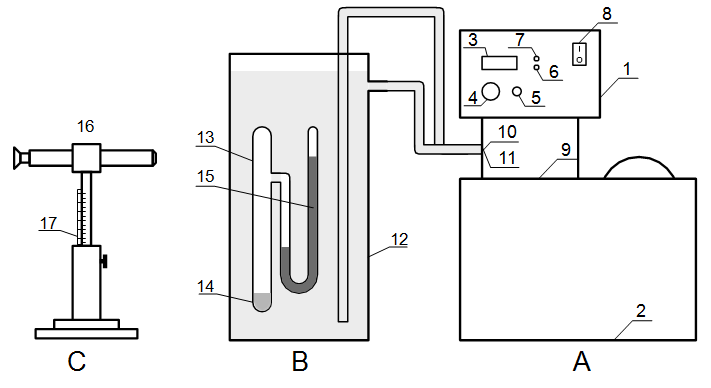
\includegraphics[scale = 0.4]{Workplace}
    \centering
\end{figure}

% Для старого измерительного прибора --- уже не актуально

% \begin{enumerate}
% \item Наполненный водой резервуар (используется в качестве термостата)
% \item Нагревательный элемент
% \item Змеевик для охлаждения воды
% \item Трубка для поступления воздуха
% \item Термометр
% \item Запаянный прибор с исследуемой жидкостью
% \end{enumerate}

\renewcommand {\labelenumi}  {\Alph{enumi}.}
\renewcommand {\labelenumii} {\arabic{enumii}.}

\begin{enumerate}
    \item Термостат
    \item Экспериментальный прибор
    \begin{enumerate}
        \setcounter {enumii}{11}
        \item Ёмкость, заполненная водой
        \item Запаянный прибор
        \item Исследуемая жидкость
        \item Манометр
    \end{enumerate}
    \item Отсчётный микроскоп
    \begin{enumerate}
        \setcounter {enumii}{15}
        \item Отсчётный микроскоп
        \item Шкала для снятия показаний с микроскопа
    \end{enumerate}
\end{enumerate}

\parag {Ход работы} ~\\

\point Включим термостат. Будем увеличивать температуру на один градус, снимать высоты $h_1$ и $h_2$ столбцов, а после находить разность высот $\Delta h$ между ними. Так же вычислим давление насыщенного пара по формуле $P = \rho_{\text{рт}} \cdot g \cdot \Delta h$, где $\rho_{\text{рт}} = 13546 ~\dfrac{\text{кг}}{\text{м}^3}$, а $g = 9,81 ~\dfrac {\text{м}}{\text{с}^2}$. Результаты занесём в таблицу \ref{tabl:up}.

\begin{table}[!h]
    \begin{tabularx}{\linewidth}{|c|X|X|X|X|X|X|X|X|}
        \hline
        $h_1$, мм & $75,00$ & $77,65$ & $77,50$ & $77,40$ & $78,25$ & $79,06$ & $80,60$ & $81,50$ \\ \hline

        $h_2$, мм & $58,50$ & $57,40$ & $56,70$ & $55,15$ & $55,45$ & $54,95$ & $53,85$ & $52,45$ \\ \hline

        $\Delta h$, мм & $16,50$ & $20,25$ & $20,80$ & $22,25$ & $22,80$ & $24,11$ & $26,75$ & $29,05$ \\ \hline

        $t$, $^o C$ & $20$ & $22$ & $23$ & $24$ & $25$ & $26$ & $27$ & $28$ \\ \hline
        
        $P$, Па & $2193$ & $2691$ & $2764$ & $2957$ & $3030$ & $3204$ & $3555$ & $3860$
        \\ \hline \multicolumn{9}{c}{} \\ \hline

        $h_1$, мм & $82,55$ & $82,95$ & $83,05$ & $84,20$ & $85,45$ & $86,20$ & $87,20$ & $88,50$ \\ \hline

        $h_2$, мм & $52,40$ & $51,90$ & $51,10$ & $50,60$ & $48,40$ & $47,35$ & $46,05$ & $45,45$ \\ \hline

        $\Delta h$, мм & $30,15$ & $31,05$ & $31,95$ & $33,60$ & $37,05$ & $38,85$ & $41,15$ & $43,05$ \\ \hline

        $t$, $^o C$ & $29$ & $30$ & $31$ & $32$ & $33$ & $34$ & $35$ & $36$ \\ \hline

        $P$, Па & $4007$ & $4126$ & $4246$ & $4465$ & $4923$ & $5163$ & $5468$ & $5721$ \\ \hline
    \end{tabularx}
\caption{Результаты измерений при увеличении температуры}
\label{tabl:up}
\end{table}

\point Сделаем те же самые измерения, уменьшая температуру. Для этого откроем кран с холодной водой так, чтобы скорость охлаждение шло примерно тем же темпом, что и нагревание. Результаты занесём в таблицу \ref{tabl:down}.

\begin{table}[!h]
    \begin{tabularx}{\linewidth}{|c|X|X|X|X|X|X|X|X|}
        \hline
        $h_1$, мм & $88,50$ & $88,15$ & $86,90$ & $85,70$ & $85,15$ & $84,85$ & $83,90$ & $81,80$ \\ \hline

        $h_2$, мм & $45,45$ & $47,80$ & $47,75$ & $49,85$ & $49,85$ & $50,70$ & $50,90$ & $51,20$ \\ \hline

        $\Delta h$, мм & $43,05$ & $40,35$ & $39,15$ & $35,85$ & $35,30$ & $34,15$ & $33,00$ & $30,60$ \\ \hline

        $t$, $^o C$ & $36$ & $35$ & $34$ & $33$ & $32$ & $31$ & $30$ & $29$ \\ \hline 
        
        $P$, Па & $5721$ & $5362$ & $5202$ & $4764$ & $4691$ & $4538$ & $4385$ & $4066$
        \\ \hline \multicolumn{9}{c}{} \\ \hline

        $h_1$, мм & $80,75$ & $80,15$ & $79,45$ & $78,50$ & $77,90$ & $76,15$ & $76,30$ & $76,00$ \\ \hline

        $h_2$, мм & $52,05$ & $52,80$ & $53,40$ & $54,10$ & $55,55$ & $55,85$ & $56,70$ & $57,20$ \\ \hline
        
        $\Delta h$, мм & $28,70$ & $27,35$ & $26,05$ & $24,40$ & $22,35$ & $20,30$ & $19,60$ & $18,80$ \\ \hline

        $t$, $^o C$ & $28$ & $27$ & $26$ & $25$ & $24$ & $23$ & $22$ & $21$ \\ \hline

        $P$, Па & $3814$ & $3634$ & $3462$ & $3242$ & $2970$ & $2698$ & $2605$ & $2498$ \\ \hline
    \end{tabularx}
\caption{Результаты измерений при уменьшении температуры}
\label{tabl:down}
\end{table}

\point Теперь построим графики зависимостей $P (T)$ и $ln P \left(\dfrac{1}{T} \right)$. График при увеличении будет обозначен красным цветом, а при уменьшении --- синим. 

\begin{figure}[!h]
    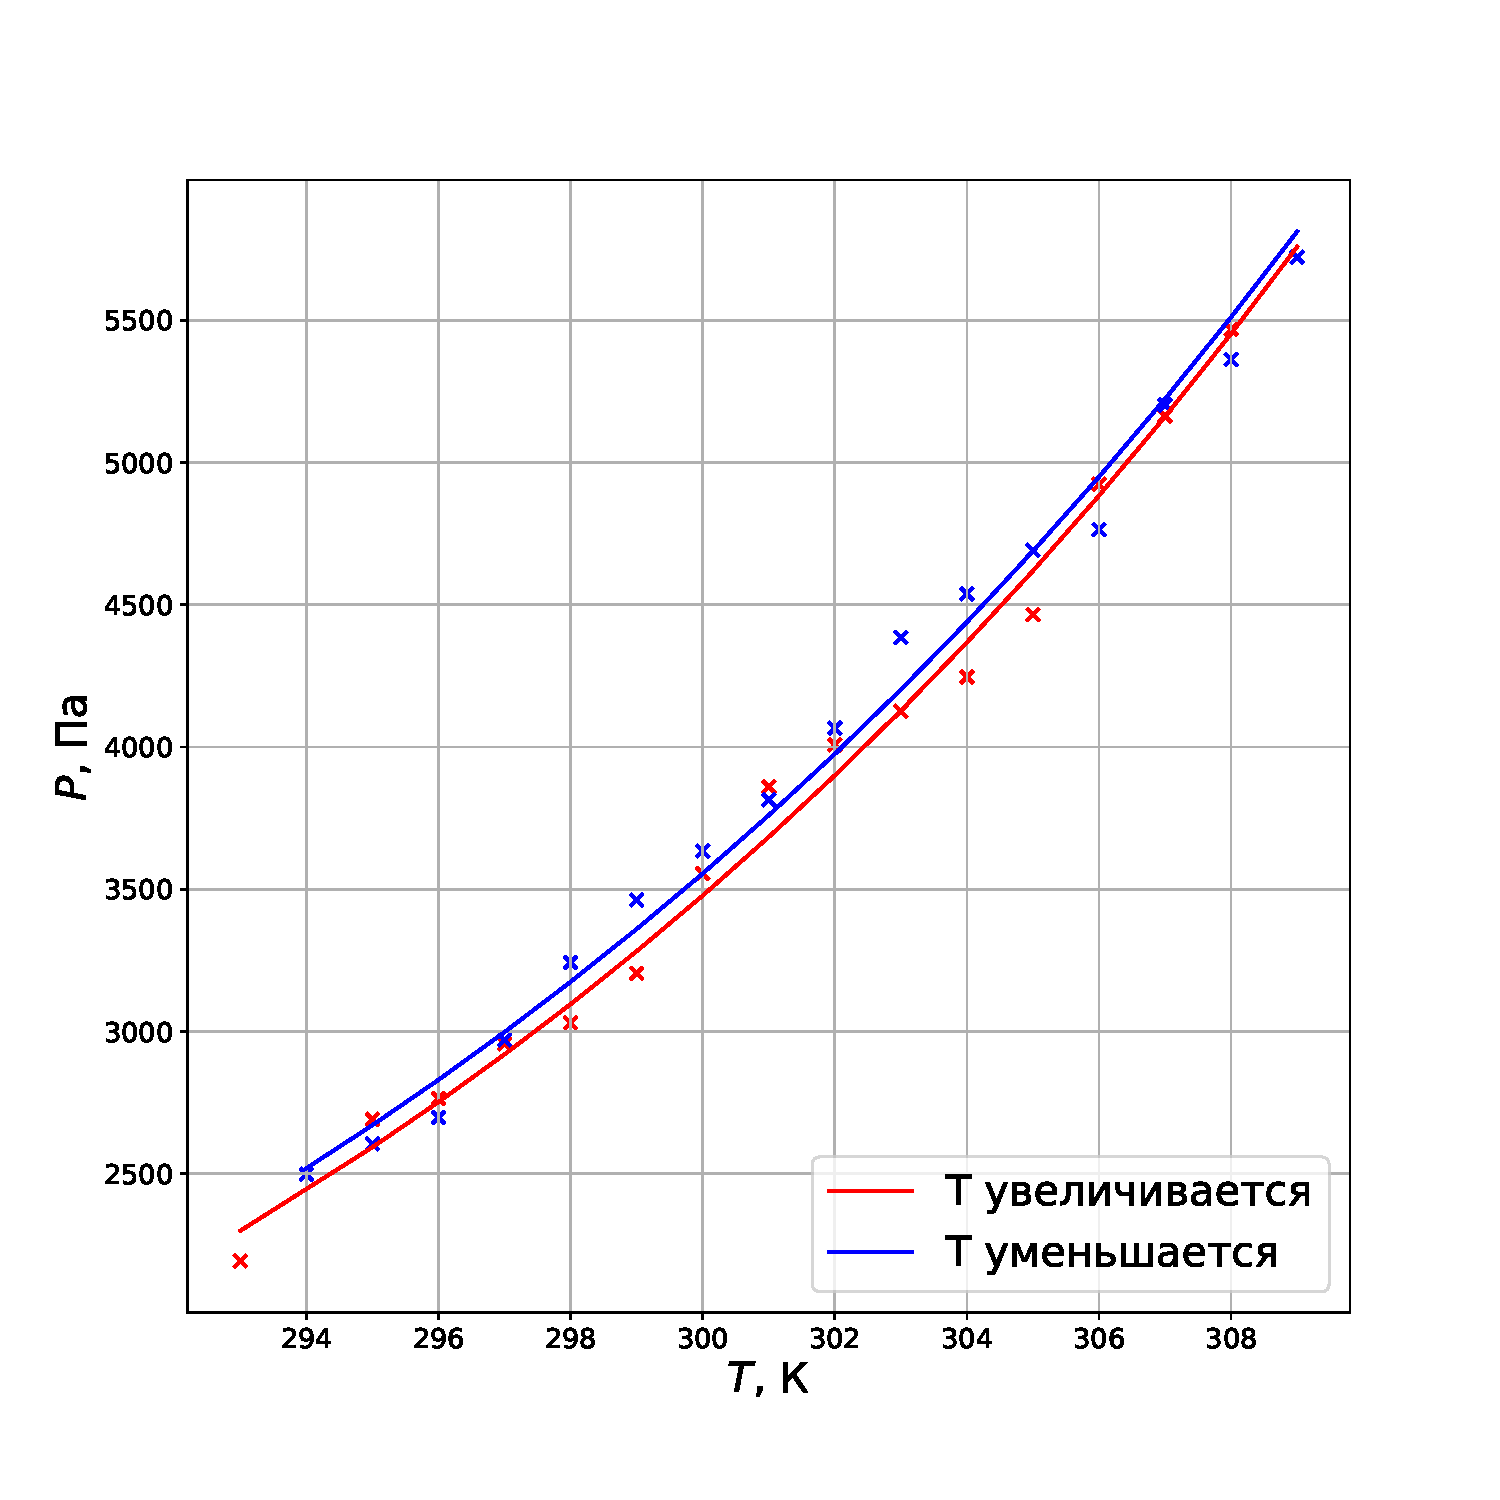
\includegraphics[scale = 0.3]{Plot1}
    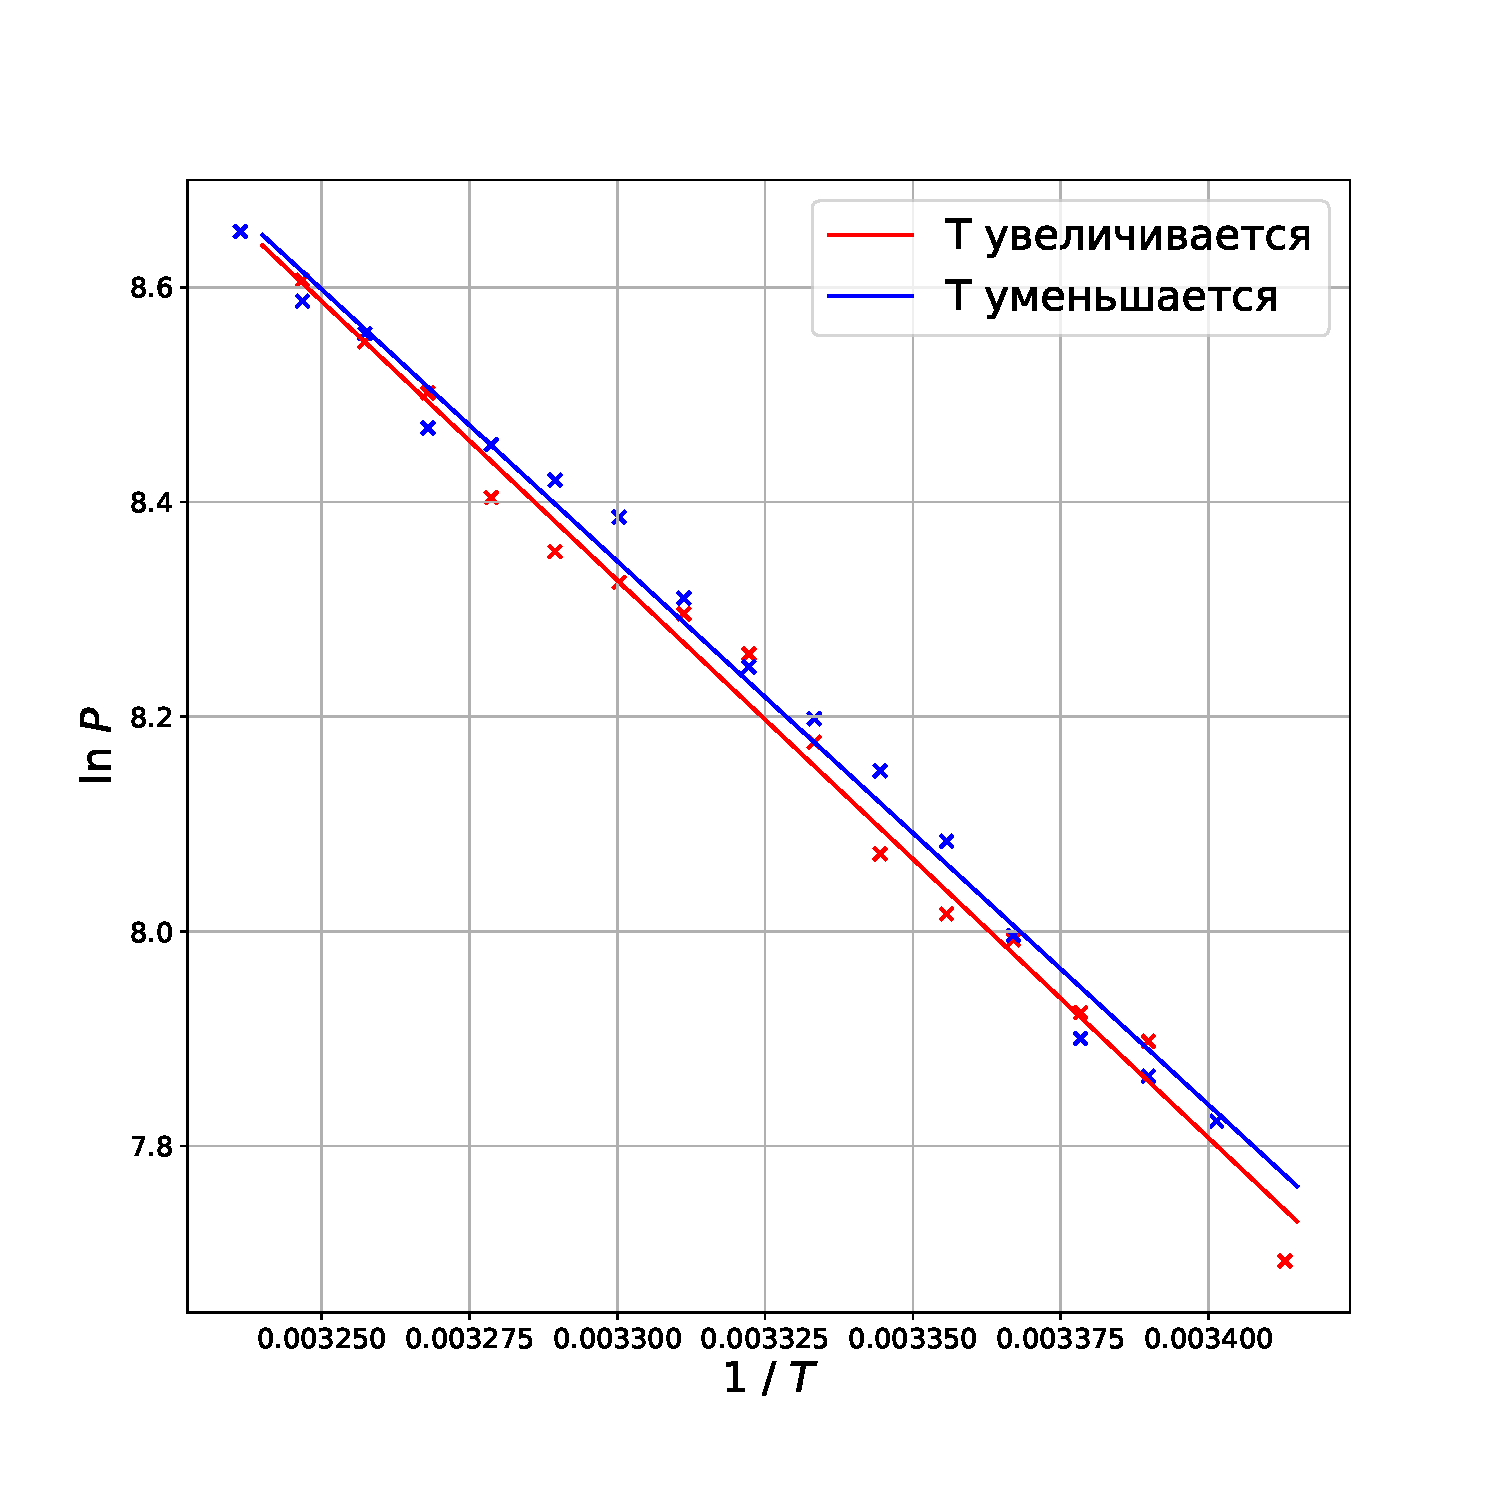
\includegraphics[scale = 0.3]{Plot2}
\end{figure}

\point Как понятно из уравнения \eqref{eq:L}, если $k$ --- коэффициент наклона графика $\ln P \left(\dfrac{1}{T} \right)$, то теплоту испарения $L$ можно вызазить следующим образом:

\begin{equation} \label{eq:L-k}
    L = -R \cdot k
\end{equation}

Т.~к. $k_{\text{ув}} = -5194$, $k_{\text{ум}} = -5063$, то получаем: $L_{\text{ув}} = 43,2  ~\dfrac{\text{кДж}}{\text{моль}}$, $L_{\text{ум}} = 42,1 ~\dfrac{\text{кДж}}{\text{моль}}$.

\vspace{0.5cm}

\point Как видно из уравнения \eqref{eq:L-k}, для погрешности $\eps_L$ верно следующее: $\eps_L = \eps_k$, а $\eps_k$ известно по формуле погрешности для МНК. Таким образом, $\eps_{L_{\text{ув}}} = 3\%$, $\eps_{L_{\text{ум}}} = 3\%$.

Табличное же значение $L$ составляет $40,7 ~\dfrac{\text{кДж}}{\text{моль}}$. Следовательно, отличие от табличного значения составляет $6\%$ и $3\%$ для увеличения и уменьшения соответственно. Значит, более точным является второй способ.

\end{document}
